% =====================================================================
% GreenFieldData MSCA Joint Doctorate -- Position L
% Candidate: Partha Pratim Saha
% v6: advertisement-aligned | APA citations | 6-page hard limit
%     Fig1=simple pipeline | Fig2=clean architecture | compact Gantt
% =====================================================================
\documentclass[11pt,a4paper]{article}

\usepackage[top=1.75cm,bottom=1.75cm,left=1.85cm,right=1.85cm]{geometry}
\usepackage{times}
\usepackage{microtype}
\usepackage{setspace}
\usepackage{titlesec}
\usepackage{enumitem}
\usepackage{graphicx}
\usepackage{booktabs}
\usepackage{array}
\usepackage{xcolor}
\usepackage{amsmath,amssymb}
\usepackage{pgfgantt}
\usepackage{multirow}
\usepackage{caption}
\usepackage{fancyhdr}
\usepackage{mdframed}
\usepackage{tabularx}
\usepackage{tikz}
\usetikzlibrary{arrows.meta,positioning,shapes.geometric,fit,calc}
\usepackage[round]{natbib}
\usepackage[T1]{fontenc}
\usepackage{hyperref}

\hypersetup{colorlinks=true,linkcolor=blue!70!black,citecolor=blue!60!black,urlcolor=teal}

\definecolor{agrigreen}{RGB}{34,139,34}
\definecolor{techblue}{RGB}{0,70,127}
\definecolor{warnorange}{RGB}{210,105,30}
\definecolor{trustpurple}{RGB}{100,40,140}
\definecolor{lightgray}{RGB}{246,246,246}
\definecolor{deepred}{RGB}{160,20,20}

\setstretch{1.18}

\titleformat{\section}{\normalsize\bfseries\color{techblue}}{}{0em}{}[\color{techblue}\titlerule]
\titleformat{\subsection}{\small\bfseries\color{agrigreen}}{}{0em}{}
\titlespacing*{\section}{0pt}{5pt}{2pt}
\titlespacing*{\subsection}{0pt}{3pt}{1pt}

\setlength{\parskip}{2pt}
\setlength{\parindent}{0pt}
\setlist[itemize]{leftmargin=1.2em,itemsep=0pt,topsep=1pt,parsep=0pt}
\setlist[enumerate]{leftmargin=1.4em,itemsep=0pt,topsep=1pt,parsep=0pt}

\pagestyle{fancy}
\fancyhf{}
\lhead{\scriptsize\textit{GreenFieldData PhD-L $|$ Partha Pratim Saha}}
\rhead{\scriptsize\textit{Calibrated Conversational Orchestration for Agricultural Robotics}}
\cfoot{\scriptsize\thepage}
\renewcommand{\headrulewidth}{0.3pt}

\newmdenv[backgroundcolor=blue!5,linecolor=techblue,linewidth=0.6pt,
  innerleftmargin=6pt,innerrightmargin=6pt,
  innertopmargin=4pt,innerbottommargin=4pt,skipabove=3pt,skipbelow=3pt]{contribbox}
\newmdenv[backgroundcolor=agrigreen!7,linecolor=agrigreen,linewidth=0.5pt,
  innerleftmargin=6pt,innerrightmargin=6pt,
  innertopmargin=3pt,innerbottommargin=3pt,skipabove=2pt,skipbelow=2pt]{scenariobox}

\begin{document}

% ---- Title Block ---------------------------------------------------
\begin{center}
{\large\bfseries\color{techblue}
  Calibrated Conversational Orchestration\\[2pt]
  for Human-Supervised Agricultural Robotic Systems}\\[4pt]
{\small\bfseries GreenFieldData MSCA Joint Doctorate --- PhD Position L}\\[2pt]
{\small Partha Pratim Saha \;$|$\; \texttt{technical.partha@gmail.com}}\\[1pt]
{\scriptsize Supervisors: Dr.\ Genoveva Vargas-Solar (CNRS/UCBLyon1) \&
Prof.\ Roberto Oberti (UniMI) \;$|$\; Submitted: 11 May 2026}
\end{center}
\vspace{-2pt}\hrule height 1pt\vspace{3pt}

% ---- Abstract ------------------------------------------------------
\begin{mdframed}[backgroundcolor=lightgray,linewidth=0.4pt,
  innerleftmargin=7pt,innerrightmargin=7pt,
  innertopmargin=4pt,innerbottommargin=4pt,skipabove=2pt,skipbelow=3pt]
\small\textbf{Abstract.}
The agricultural robotics market is growing from \$5.9B (2022) to \$11.9B projected by 2026 \citep{phd_adv_2026}---yet current IoRT (Internet of Robotic Things) control interfaces presuppose programming-level expertise, excluding the agronomists who are legally accountable for field decisions. \textbf{AgriTalk} proposes a calibrated conversational orchestration layer: four scientifically grounded contributions address (i)~NL intent compilation with statistically principled conformal-prediction uncertainty and HITL trigger policies, (ii)~verifiably faithful explanation through Belief Vector Field geometry---the candidate's own prior work---rather than unreliable Chain-of-Thought, (iii)~atomic temporal grounding against live IoT field state via streaming aggregation, and (iv)~an empirical collaborative trust evaluation framework. Together they produce a human-auditable, GDPR-aligned, Metaflow-reproducible conversational layer for precision pesticide spraying---with non-bypassable safety gates.
\end{mdframed}

% =====================================================================
\section*{Introduction and Research Context}
% =====================================================================

\textbf{Programme context.}
GreenFieldData (HORIZON MSCA Joint Doctoral Network) trains researchers to tackle digital and green transition challenges in sustainable agriculture through IoRT-based solutions \citep{phd_adv_2026}.
Position~L---supervised by Dr.\ Vargas-Solar (distributed data management, conversational analytics~\citep{vargas_solar_2021}) and Prof.\ Oberti (precision crop protection, agricultural robotics)---targets NL interfaces over robotic and analytical farming systems.
Agricultural robots (weeding, spraying, seeding, harvesting, autonomous tractors, drones) cooperate in multi-modal IoRT systems requiring IoT data collection, streaming analytics, computer vision, cloud computing, and AI.
Yet current platforms presuppose programmer-level expertise: farmers and agronomists---who are legally accountable for pesticide use, spray drift compliance, and crop safety---cannot directly command or supervise the systems they depend on \citep{chen_2021,wagner_2025}.
\textbf{AgriTalk} addresses this by creating a unified conversational layer where end-users express high-level agricultural tasks in natural language, dynamically mapped to calibrated, explainable, and auditable IoRT control processes---transforming robotic spraying from reactive and ad-hoc to knowledge-driven, safe, and operator-supervised.

\textbf{Four scientific gaps driving AgriTalk:}
\textbf{(G1)~NL disambiguation:} agricultural commands are contextually under-specified and temporally conditional---a single utterance conflates spatial reference, dosage, chemical identity, phenological timing, and weather constraints, requiring calibrated disambiguation beyond slot-filling NLU \citep{chen_2021}.
\textbf{(G2)~Calibration and explanation:} LLM softmax confidence is systematically overconfident on out-of-distribution inputs \citep{guo_calibration_2017}; Chain-of-Thought rationales are behaviorally generated, not computationally causal---anthropomorphizing them as transparent cognition produces dangerously misleading safety evaluations \citep{turpin_2023,kambhampati_2025}.
\textbf{(G3)~Temporal IoT grounding:} heterogeneous field streams must be atomically consistent for command grounding---no system currently solves this at agronomic granularity \citep{vargas_solar_2021}.
\textbf{(G4)~Trust calibration:} the causal link between faithful explanation and operator trust in HITL\footnote{HITL: Human-in-the-Loop---deliberate inclusion of human judgment before robot actuation.} agricultural systems is empirically unmeasured.

\begin{scenariobox}
\small\textbf{Focal Scenario.}
\emph{``Spray more pesticide on the struggling section near the east boundary.''}
Simultaneous ambiguities: spatial reference (which east boundary?), dosage baseline (more than what?), chemical formulation (resistance profiles + phenological stage), spray drift legality (current wind speed). Wrong interpretation: crop destruction, regulatory violation. Over-confirmation: alert fatigue. AgriTalk resolves this with calibrated statistical confidence, verifiable attribution, and an immutable audit trail.
\end{scenariobox}

% =====================================================================
\section{Research Questions and Contributions}
% =====================================================================

\noindent\textbf{Research question breakdown} (objective, data, expected output, PhD contribution):

\begin{center}
\setlength{\tabcolsep}{3pt}\scriptsize
\begin{tabularx}{\linewidth}{@{}p{0.48cm}p{2.65cm}p{2.25cm}p{2.55cm}X@{}}
\toprule
\textbf{RQ} & \textbf{Objective} & \textbf{Input Data} & \textbf{Expected Output} & \textbf{PhD Contribution} \\
\midrule
\textbf{RQ1} & Derive statistically valid HITL trigger policies from conformal NL intent calibration under seasonal distribution shift & AgroNLP corpus (labelled commands); seasonal calibration holdouts; conformal scores & Coverage-certified $\mathcal{C}(x)$; adaptive HITL policy per action class; ECE vs.\ softmax baseline & C1: first principled uncertainty-to-HITL mapping for safety-critical agricultural NL commands \\[3pt]
\textbf{RQ2} & Provide verifiably faithful attribution by tracing BVF\footnote{BVF: Belief Vector Field---layer-wise geometric trajectory of model representational state \citep{saha_bvf_2026}.} geometry, not generating CoT narratives & Fine-tuned LLM layer activations; IG, LRP, SHAP, rollout, BVF; operator study (N$\geq$30) & BVF layer traces; cross-method Kendall~$\tau$; trust calibration gap $\Delta$(C vs.\ B) & C2: BVF as computationally causal alternative to CoT---empirically tested not assumed \\[3pt]
\textbf{RQ3} & Enable real-time atomic NL grounding against IoT field state; characterize failure under sensor degradation & Kafka streams (sensor, NDVI, weather, telemetry); fault injection; Gazebo simulation & Time-indexed field-state register; recall vs.\ degradation curve; V2 staleness alerts & C3: first atomic conversational grounding layer for agricultural IoRT at stream granularity \\[3pt]
\textbf{RQ4} & Measure whether faithful attribution causally improves trust calibration vs.\ CoT; build reusable evaluation protocol & 3-condition user study; HITL trace logs; trust surveys; Metaflow seasonal replay & CTEF protocol; trust gap $\Delta$; seasonal reproducibility archive; NASA-TLX & C4: closes empirical loop between explanation faithfulness and operator trust calibration \\
\bottomrule
\end{tabularx}
\end{center}

\smallskip
\begin{contribbox}
\small\textbf{Four primary research contributions:}\\[-5pt]
\begin{itemize}
\item[\textbf{C1}] \textbf{[AI Safety] Calibrated Intent Compiler (CIC):} Conformal prediction-based NL-to-command compilation with statistically guaranteed HITL trigger policies (EMNLP/ACL 2027).
\item[\textbf{C2}] \textbf{[Interpretability] Belief-Grounded Explanation System (BGES):} BVF layer-wise geometry for verifiably faithful attribution, validated by a human operator study (ACL/EMNLP 2028; FAccT 2029).
\item[\textbf{C3}] \textbf{[Streaming NLP] Temporal Streaming Grounding Aggregator (TSGA):} Atomically consistent time-indexed field-state register for contextual grounding under sensor uncertainty (Computers \& Electronics in Agriculture Q1 2028 or VLDB 2028).
\item[\textbf{C4}] \textbf{[Collaborative Trust] Collaborative Trust Evaluation Framework (CTEF):} Mixed-methods framework measuring how calibrated uncertainty and faithful attribution causally improve operator trust (CHI 2029 or FAccT 2029).
\end{itemize}
\end{contribbox}

% =====================================================================
\section{System Architecture: AgriTalk}
% =====================================================================

% ---- Figure 1: Simple 4-stage pipeline (easy to explain at interview) ----
\begin{figure}[!h]
\centering
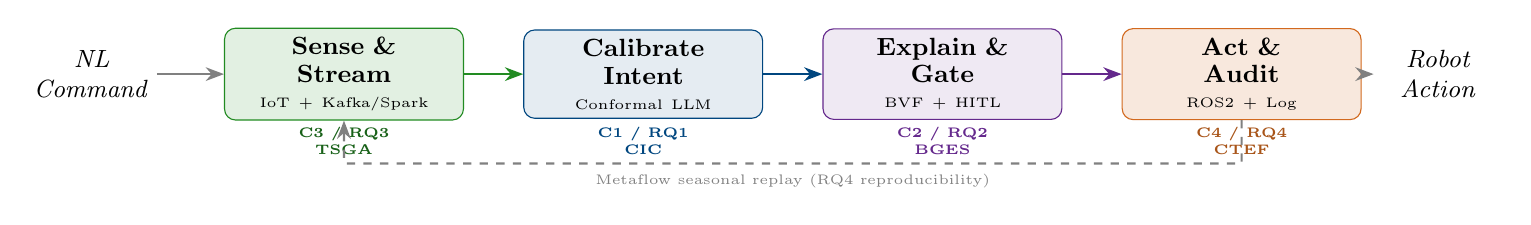
\begin{tikzpicture}[font=\small, >=Stealth,
  stage/.style={draw, rounded corners=4pt, minimum width=3.0cm,
    minimum height=0.9cm, align=center, text width=2.8cm},
  clbl/.style={font=\tiny\bfseries, align=center}]
% Input label
\node[font=\small\itshape, align=center, text width=1.4cm] (nl)
  at (0, 0) {NL\\Command};
% Four stage boxes
\node[stage, fill=agrigreen!13, draw=agrigreen]     (s1) at (3.2,  0)
  {\textbf{Sense \&}\\[-1pt]\textbf{Stream}\\[-2pt]{\tiny IoT + Kafka/Spark}};
\node[stage, fill=techblue!10,  draw=techblue]       (s2) at (7.0,  0)
  {\textbf{Calibrate}\\[-1pt]\textbf{Intent}\\[-2pt]{\tiny Conformal LLM}};
\node[stage, fill=trustpurple!10,draw=trustpurple]   (s3) at (10.8, 0)
  {\textbf{Explain \&}\\[-1pt]\textbf{Gate}\\[-2pt]{\tiny BVF + HITL}};
\node[stage, fill=warnorange!15, draw=warnorange]    (s4) at (14.6, 0)
  {\textbf{Act \&}\\[-1pt]\textbf{Audit}\\[-2pt]{\tiny ROS2 + Log}};
% Output label
\node[font=\small\itshape, align=center, text width=1.4cm] (robot)
  at (17.1, 0) {Robot\\Action};
% Arrows between stages
\draw[->, thick, gray]         (nl.east)  -- (s1.west);
\draw[->, thick, agrigreen]    (s1.east)  -- (s2.west);
\draw[->, thick, techblue]     (s2.east)  -- (s3.west);
\draw[->, thick, trustpurple]  (s3.east)  -- (s4.west);
\draw[->, thick, gray]         (s4.east)  -- (robot.west);
% Contribution labels below each box
\node[clbl, text=agrigreen!70!black] at (3.2,  -0.85) {C3 / RQ3\\TSGA};
\node[clbl, text=techblue]           at (7.0,  -0.85) {C1 / RQ1\\CIC};
\node[clbl, text=trustpurple]        at (10.8, -0.85) {C2 / RQ2\\BGES};
\node[clbl, text=warnorange!80!black]at (14.6, -0.85) {C4 / RQ4\\CTEF};
% Metaflow feedback arc
\draw[->, dashed, gray, thick]
  (s4.south) -- ++(0,-0.55)
  -- node[below, font=\tiny, gray]{Metaflow seasonal replay (RQ4 reproducibility)}
  ++(-11.4,0) -- (s1.south);
\end{tikzpicture}
\vspace{-4pt}
\caption{\scriptsize\textbf{AgriTalk: four-stage conversational orchestration pipeline (Figure 1).}
Each stage maps to one research contribution and one information boundary group.
The dashed arc is the Metaflow artifact replay path: archived sensor snapshots and model checkpoints from Year~1 (Lyon) can be re-executed on Year~2 (Milan) context, making RQ4 trust measurements reproducible and season-comparable without re-running real experiments.}
\label{fig:pipeline}
\end{figure}

\textbf{Information boundaries and verifier layer.}
Acronyms: NDVI = Normalized Difference Vegetation Index (crop health; value $<$0.35 indicates stress zone); DQ = Data Quality (V1 verifier: freshness, completeness, cross-modality consistency); JWT = JSON Web Token (cryptographically signed auth); RBAC = Role-Based Access Control; ROS2 = Robot Operating System~2 (DDS middleware); KB = Knowledge Base (EPPO/PPDB agronomic records: spray drift limits, dosage protocols, resistance profiles).
AgriTalk crosses five information boundaries (B1--B5), each guarded by a dedicated verifier (V1--V5).
The HITL gate (V5) is architecturally non-bypassable: five trigger conditions---action type in \{SPRAY, ABORT, DOSAGE\_CHANGE, ZONE\_OVERRIDE, EMERGENCY\_STOP\}, $|\mathcal{C}(x)|\geq 2$, unverified KB entity, DQ failure, or role = OBSERVER---must be cleared before robot actuation. No API pathway overrides this.

% ---- Figure 2: Clean vertical architecture ----
\begin{figure}[!h]
\centering
\resizebox{\linewidth}{!}{%
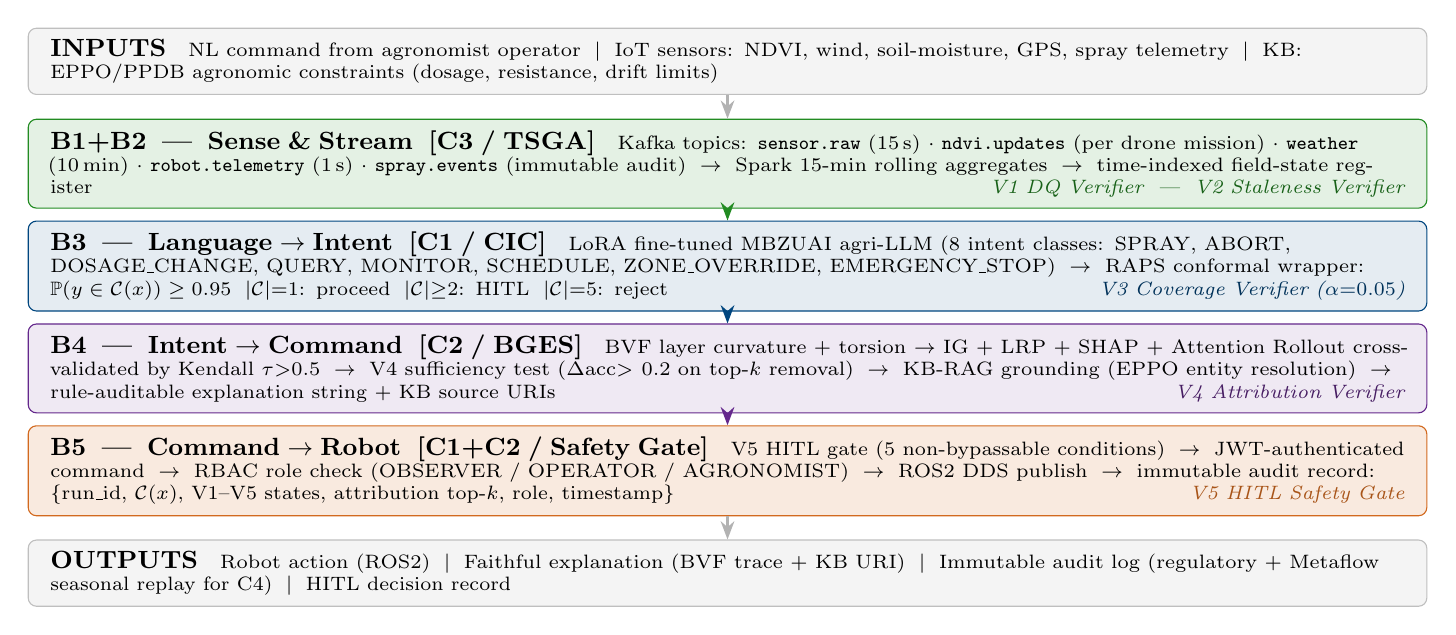
\begin{tikzpicture}[font=\scriptsize, >=Stealth,
  blk/.style={draw, rounded corners=3pt,
    minimum width=17.5cm, minimum height=0.68cm,
    align=left, inner xsep=8pt, inner ysep=4pt,
    text width=17.2cm}]
% ---- tiers (top to bottom) ----
\node[blk, fill=gray!9, draw=gray!50] (inp) at (0, 7.1)
  {\textbf{\small INPUTS}\quad NL command from agronomist operator
   \;\textbar\; IoT sensors: NDVI, wind, soil-moisture, GPS, spray telemetry
   \;\textbar\; KB: EPPO/PPDB agronomic constraints (dosage, resistance, drift limits)};

\node[blk, fill=agrigreen!12, draw=agrigreen] (b12) at (0, 5.8)
  {\textbf{\small B1+B2 \;|\; Sense \& Stream \;[C3 / TSGA]}\quad
   Kafka topics:
   \texttt{sensor.raw} (15\,s) $\cdot$ \texttt{ndvi.updates} (per drone mission)
   $\cdot$ \texttt{weather} (10\,min) $\cdot$ \texttt{robot.telemetry} (1\,s)
   $\cdot$ \texttt{spray.events} (immutable audit) \;$\to$\;
   Spark 15-min rolling aggregates \;$\to$\; time-indexed field-state register
   \hfill\normalfont\textit{\color{agrigreen!70!black}V1 DQ Verifier \;|\; V2 Staleness Verifier}};

\node[blk, fill=techblue!10, draw=techblue] (b3) at (0, 4.5)
  {\textbf{\small B3 \;|\; Language $\to$ Intent \;[C1 / CIC]}\quad
   LoRA fine-tuned MBZUAI agri-LLM (8 intent classes: SPRAY, ABORT, DOSAGE\_CHANGE, QUERY, MONITOR, SCHEDULE, ZONE\_OVERRIDE, EMERGENCY\_STOP) \;$\to$\;
   RAPS conformal wrapper: $\mathbb{P}(y\in\mathcal{C}(x))\geq 0.95$\;
   $|\mathcal{C}|{=}1$: proceed \;$|\mathcal{C}|{\geq}2$: HITL \;$|\mathcal{C}|{=}5$: reject
   \hfill\normalfont\textit{\color{techblue!70!black}V3 Coverage Verifier ($\alpha{=}0.05$)}};

\node[blk, fill=trustpurple!10, draw=trustpurple] (b4) at (0, 3.2)
  {\textbf{\small B4 \;|\; Intent $\to$ Command \;[C2 / BGES]}\quad
   BVF layer curvature + torsion $\to$ IG + LRP + SHAP + Attention Rollout
   cross-validated by Kendall~$\tau{>}0.5$ \;$\to$\;
   V4 sufficiency test ($\Delta$acc$>0.2$ on top-$k$ removal) \;$\to$\;
   KB-RAG grounding (EPPO entity resolution) \;$\to$\; rule-auditable explanation string + KB source URIs
   \hfill\normalfont\textit{\color{trustpurple!70!black}V4 Attribution Verifier}};

\node[blk, fill=warnorange!14, draw=warnorange] (b5) at (0, 1.9)
  {\textbf{\small B5 \;|\; Command $\to$ Robot \;[C1+C2 / Safety Gate]}\quad
   V5 HITL gate (5 non-bypassable conditions) \;$\to$\;
   JWT-authenticated command \;$\to$\; RBAC role check (OBSERVER / OPERATOR / AGRONOMIST) \;$\to$\;
   ROS2 DDS publish \;$\to$\; immutable audit record:
   \{run\_id, $\mathcal{C}(x)$, V1--V5 states, attribution top-$k$, role, timestamp\}
   \hfill\normalfont\textit{\color{warnorange!80!black}V5 HITL Safety Gate}};

\node[blk, fill=gray!9, draw=gray!50] (out) at (0, 0.6)
  {\textbf{\small OUTPUTS}\quad Robot action (ROS2)
   \;\textbar\; Faithful explanation (BVF trace + KB URI)
   \;\textbar\; Immutable audit log (regulatory + Metaflow seasonal replay for C4)
   \;\textbar\; HITL decision record};

% ---- vertical flow arrows ----
\draw[->, thick, gray!60]      (inp.south)  -- (b12.north);
\draw[->, thick, agrigreen]    (b12.south)  -- (b3.north);
\draw[->, thick, techblue]     (b3.south)   -- (b4.north);
\draw[->, thick, trustpurple]  (b4.south)   -- (b5.north);
\draw[->, thick, gray!60]      (b5.south)   -- (out.north);
\end{tikzpicture}%
}
\vspace{-4pt}
\caption{\scriptsize\textbf{AgriTalk 5-boundary system architecture (Figure 2).}
Each horizontal tier is one information boundary.
Color: \textcolor{agrigreen}{green} = streaming data management (C3); \textcolor{techblue}{blue} = calibrated intent (C1); \textcolor{trustpurple}{purple} = attribution/explanation (C2); \textcolor{warnorange}{orange} = safety gate (C1+C2).
Every tier emits a verifiable artifact; V5's immutable audit record is both the regulatory accountability anchor and the scientific data substrate for C4 (CTEF) seasonal trust measurement.}
\label{fig:arch}
\end{figure}

% =====================================================================
\section{Methods and Experiments}
% =====================================================================

\textbf{C1 -- Calibrated Intent Compiler (RQ1).}
The AgroNLP corpus is built via structured agronomist interviews (5--8 experts at UCBLyon1 partner farms) producing intent-labelled commands across 8 classes; the safety-critical \texttt{ABORT} class ($\approx$2\% of natural distribution) is handled by stratified sampling and asymmetric focal loss, with seasonal cohort splitting (Lyon Year~1 $\to$ Milan Year~2) preventing temporal data leakage.
LoRA fine-tuning adapts the MBZUAI agricultural LLM\footnote{\scriptsize\texttt{MBZUAI/agriculture-llm}, HuggingFace.}; RAPS conformal wrapping \citep{angelopoulos_2023} delivers per-class coverage $\mathbb{P}(y\in\mathcal{C}(x))\geq 0.95$.
\textit{Core open question (RQ1):} does exchangeability hold under seasonal drift?
Experiments: (a)~coverage stability (Year~2 test vs.\ Year~1 calibration sets); (b)~HITL policy ablation (conformal-triggered vs.\ softmax-threshold vs.\ always-HITL); (c)~Gazebo fault injection.
ECE\footnote{ECE: average deviation between model confidence and empirical accuracy across bins \citep{guo_calibration_2017}.} monitors calibration quality; V3 triggers recalibration when coverage degrades $>$0.02.
Novel parameter extraction from EPPO/PPDB manuals (spray dosage, resistance profiles) is embedded as KB grounding---transforming robotic spraying from ad-hoc to knowledge-driven \citep{phd_adv_2026}.

\textbf{C2 -- Belief-Grounded Explanation System (RQ2).}
CoT traces are behavioral outputs, not computational records---systematically unfaithful to the model's actual processing \citep{turpin_2023,kambhampati_2025,oxford_cot_2025}.
BVF \citep{saha_bvf_2026} traces layer-wise representational geometry: syntactic (verb/object, early layers) $\to$ semantic (``struggling section'' = NDVI$<$0.35?, mid layers) $\to$ agronomic safety (dosage within EPPO limits?, late layers)---a verifiable computational pathway.
Five attribution methods (IG~\citep{sundararajan_ig_2017}, LRP~\citep{bach_lrp_2015}, SHAP~\citep{lundberg_shap_2017}, Attention Rollout~\citep{abnar_attention_2020}, BVF) are cross-validated by Kendall~$\tau$ and V4 sufficiency/necessity tests.
A 3-condition between-subjects operator study (N$\geq$30, Year~2, UniMI): \textbf{A}~no explanation; \textbf{B}~CoT narrative; \textbf{C}~faithful BVF + KB URI string.
Primary measure: trust calibration gap $\Delta$ (perceived minus empirical reliability); analysis: Wilcoxon signed-rank, Cohen's~$d$, NASA-TLX cognitive workload (faithful explanation must not overload operators).
This realises the advertisement objective of stakeholder empowerment through natural language corrections aligned to expert knowledge, with human-AI co-evolution of robot behaviour \citep{phd_adv_2026}.

\textbf{C3 -- Temporal Streaming Grounding Aggregator (RQ3).}
TSGA maintains a time-indexed field-state register: Kafka topics (\texttt{sensor.raw} 15\,s; \texttt{ndvi.updates} per mission; \texttt{weather} 10\,min; \texttt{telemetry} 1\,s; \texttt{spray.events} immutable) with Avro schema registry; Spark Structured Streaming applies 15-min rolling aggregates.
Grounding uses the exact register snapshot at query receipt time---resolving temporal ambiguity: ``spray now'' uses the live register; ``was Tuesday safe?'' uses the Metaflow-archived artifact from that timestamp.
Failure boundary experiments: sensor dropout (10--50\%), telemetry lag ($>$5\,min), GPS/vision conflict---characterising connectivity-limited rural farm risk rather than assuming reliable IoT.
This directly implements the advertisement's objective of conversa\-tional streaming dataflow orchestration \citep{phd_adv_2026}.

\textbf{C4 -- Collaborative Trust Evaluation Framework (RQ4).}
CTEF operationalises \textit{collaborative trust}: the operator's calibrated confidence in AI outputs measured as willingness to act while retaining situational authority.
Four instruments: (1)~pre/post trust calibration survey; (2)~behavioral trace analysis (HITL decisions per explanation condition); (3)~think-aloud protocol; (4)~Metaflow seasonal replay---re-running archived pipeline steps on historical snapshots to test cross-season policy generalization.
Statistical analysis: Wilcoxon signed-rank, Cohen's~$d$, regression controlling for role and experience.
All pipeline artifacts are immutably versioned: \{run\_id, git\_sha, artifact\_hash, season\_label, farm\_id\}---the scientific infrastructure making RQ4 answerable across seasons and farms.
Three deployment tiers: \textit{local} (UCBLyon1 GPU, fine-tuning), \textit{edge} (NVIDIA Jetson AGX Orin, 8-bit quantized, P95 latency $<$800\,ms), \textit{cloud} (Azure/\texttt{@kubernetes}, federated C4 replay).

% =====================================================================
\section{Evaluation Framework and Datasets}
% =====================================================================

\begin{center}\small
\begin{tabularx}{\linewidth}{@{}lXl@{}}
\toprule
\textbf{Metric} & \textbf{Justification} & \textbf{Target} \\
\midrule
Macro-F1 (intent)      & Multi-class imbalance; ABORT rare but asymmetrically costly \citep{chen_2021} & $\geq$ baseline \\
ECE (calibration)      & Overconfidence vs.\ softmax \citep{guo_calibration_2017}; trust requires reliable confidence & $<$ softmax ECE \\
ABORT recall           & Type-II error catastrophic; safety-critical class & Maximize \\
Coverage stability     & Conformal drift under seasonal shift; recalibration trigger & Monitor \\
Kendall $\tau$(IG,LRP) & Cross-method attribution agreement; faithfulness signal & $\tau>0.5$ \\
Trust calibration gap  & Perceived $-$ empirical reliability; condition C vs.\ B & $\Delta$(C$-$B)$<0$ \\
NASA-TLX workload      & Faithful explanation must not overload practitioners & Non-inferior to B \\
Edge P95 latency       & ABORT safety on Jetson AGX Orin deployment & $<$800\,ms \\
\bottomrule
\end{tabularx}
\end{center}

\smallskip
\begin{center}\small
\begin{tabularx}{\linewidth}{@{}p{0.55cm}p{2.1cm}Xp{2.3cm}@{}}
\toprule
\textbf{Year} & \textbf{Institution} & \textbf{Datasets and Sources} & \textbf{Purpose} \\
\midrule
\textbf{Y1} & UCBLyon1 & AgroNLP corpus (novel, agronomist interviews); PANGAEA soil/crop records; MBZUAI agri-LLM (HuggingFace, fine-tuning base); ACRE precision benchmark; OpenWeather Lyon 2020--2026 API & C1 corpus construction; C3 grounding baseline; LLM fine-tuning \\[2pt]
\textbf{Y2} & UniMI\,+\,ProBayes & ProBayes partner farm logs (GDPR-compliant, federated); UniMI experimental spray records; FieldRobot Event 2026/2027 simulation; EPPO/PPDB live API; USDA-ARS-AgAID farmland\_agriculture (HuggingFace) & C2 operator study; C3 failure boundary; real-robot validation \\[2pt]
\textbf{Y3} & Both & Cross-farm federated corpus (2--4 farms, CFL \citep{saha_cfl_2024}); synthetic adversarial corpus; Metaflow seasonal replay artifacts & C4 trust evaluation; generalization; CTEF reproducibility \\
\bottomrule
\end{tabularx}
\end{center}

% =====================================================================
\section{Three-Year Roadmap and Expected Outcomes}
% =====================================================================

\begin{center}
\resizebox{\linewidth}{!}{%
\begin{ganttchart}[
    hgrid,
    vgrid={*1{draw=white}},
    bar/.append style={fill=techblue!35, rounded corners=1pt},
    bar label font=\small,
    group label font=\small\bfseries,
    milestone label font=\small\itshape,
    title label font=\small\bfseries,
    title height=0.7,
    x unit=0.54cm,
    y unit chart=0.50cm]{1}{36}
  % Year-level title bars (no monthly breakdown)
  \gantttitle{Year 1 \;|\; UCBLyon1 \;(Oct 2026 -- Sep 2027)}{12}
  \gantttitle{Year 2 \;|\; UniMI + ProBayes \;(Oct 2027 -- Sep 2028)}{12}
  \gantttitle{Year 3 \;|\; Both Institutions \;(Oct 2028 -- Sep 2029)}{12} \\
  % Year 1 activities
  \ganttbar[bar/.append style={fill=techblue!25}]{Literature review \& SotA}{1}{3} \\
  \ganttbar[bar/.append style={fill=agrigreen!45}]{AgroNLP corpus: interviews + annotation (C1)}{2}{7} \\
  \ganttbar[bar/.append style={fill=techblue!40}]{LLM fine-tuning + conformal calibration (C1)}{5}{10} \\
  \ganttmilestone{\textit{C1 $\to$ EMNLP / ACL 2027}}{11} \\
  % Year 2 activities
  \ganttbar[bar/.append style={fill=warnorange!40}]{ProBayes adaptive calibration + partner integration}{13}{17} \\
  \ganttbar[bar/.append style={fill=agrigreen!50}]{Streaming TSGA: Kafka/Spark + Gazebo (C3)}{14}{20} \\
  \ganttbar[bar/.append style={fill=trustpurple!40}]{BVF attribution + BGES implementation (C2)}{19}{24} \\
  \ganttbar[bar/.append style={fill=warnorange!35}]{User study protocol + IRB approval}{22}{24} \\
  \ganttmilestone{\textit{C3 $\to$ C\&E Agriculture / VLDB 2028}}{24} \\
  % Year 3 activities
  \ganttbar[bar/.append style={fill=warnorange!50}]{HITL operator study: 3-condition (A/B/C)}{25}{29} \\
  \ganttbar[bar/.append style={fill=trustpurple!45}]{CTEF + RQ4 trust analysis + seasonal replay (C4)}{28}{33} \\
  \ganttbar[bar/.append style={fill=techblue!30}]{Thesis writing + revisions}{31}{36} \\
  \ganttmilestone{\textit{C2+C4 $\to$ ACL / FAccT 2029}}{32} \\
  \ganttmilestone{\textbf{PhD Defence}}{36}
\end{ganttchart}%
}
\end{center}
\vspace{2pt}

\textbf{Expected outcomes:} (1)~3 peer-reviewed publications (C1/EMNLP 2027, C3/CEA-VLDB 2028, C2+C4/CHI-FAccT 2029); (2)~open-source AgriTalk prototype (Metaflow pipelines, conformal module, BVF layer); (3)~AgroNLP benchmark corpus (public release); (4)~CTEF evaluation protocol (reusable beyond this project); (5)~complete Metaflow artifact archive for seasonal replay.

\begin{center}\small
\begin{tabularx}{\linewidth}{@{}lXX@{}}
\toprule
\textbf{Risk} & \textbf{Primary Plan} & \textbf{Backup} \\
\midrule
Real robot access delayed     & Gazebo simulation (Months 1--18); all C1/C3 papers feasible on sim + ACRE & Robot needed only for C2 user study + real spray logs \\
Corpus too small              & Agronomist interviews + expert-validated synthetic commands & MultiWOZ agricultural domain transfer \\
Conformal coverage drifts     & Adaptive recalibration; per-season calibration checkpoints & Conservative fixed threshold; full HITL fallback \\
BVF over-smoothing at depth   & Multi-layer torsion analysis; curvature monitoring & SHAP + LRP primary; BVF as supplementary analysis \\
\bottomrule
\end{tabularx}
\end{center}

% =====================================================================
\section{Responsible AI, Design Choices, and Candidature}
% =====================================================================

\textbf{Responsible AI by design.}
\textbf{(1)~Safety-by-architecture:} V5 HITL gate is non-bypassable; \texttt{ABORT} requires AGRONOMIST role; no code pathway can override it.
\textbf{(2)~Explainability before actuation:} V4 attribution verifier runs \emph{before} command execution---explanation is a gate, not an audit footnote.
\textbf{(3)~Privacy / GDPR:} federated CFL \citep{saha_cfl_2024} ensures raw farm data never leaves the farm; differential privacy on cross-farm aggregation.
\textbf{(4)~Failure transparency:} all V1--V5 failures surface with explicit, audit-logged reason codes (DQ channel, staleness duration, coverage shortfall, attribution disagreement, latency violation)---no silent degradation.
\textbf{(5)~Operator autonomy:} HITL design intentionally preserves human situational authority; AgriTalk assists---it does not automate away agronomist judgment.

\textbf{Design rationale.}
\textit{Conformal prediction over Bayesian calibration:} distribution-free coverage from a single calibration pass---tractable at 800\,ms edge inference without MCMC \citep{angelopoulos_2023,shafer_vovk_2008}.
\textit{BVF over CoT:} faithfulness is a testable empirical claim (RQ2), not a design preference.
\textit{Open models:} gradient access for attribution; reproducible on UCBLyon1 GPU without API costs.
\textit{Simulation-first:} Year~1 Gazebo $\to$ Year~2 real robot under Prof.\ Oberti---honest scoping; this is a conversational AI PhD, not a robotics hardware project.

\textbf{Candidature.}
My ongoing BVF research \citep{saha_bvf_2026} provides direct grounding in layer-wise attribution and over-smoothing artifacts (C2); CFL work \citep{saha_cfl_2024} is the direct basis for Year~3 cross-farm generalization (C3 extension).
Teaching AI and IoT to 50+ student projects built practical understanding of sensor deployment and non-specialist explanation design essential for the C4 user study.
Supervision aligns precisely: Dr.\ Vargas-Solar (streaming data management, DAG orchestration, conversational analytics) $\to$ C3/C4; Prof.\ Oberti (precision agriculture, field validation, spray robotics) $\to$ C1/C2 operator study.
The open questions I find most compelling---whether conformal coverage survives seasonal distribution drift, and whether faithful attribution measurably improves trust calibration or merely overwhelms operators---are exactly why this is a PhD and not an engineering project.

\textit{Note on AI assistance:} this proposal was drafted with AI writing tools. All research design, scientific choices, critical analysis, and design rationale are the candidate's own intellectual work, fully defensible at interview.

% =====================================================================
\bibliographystyle{apalike}
\bibliography{proposal_refs}
\end{document}
